% !TeX spellcheck = cs_CZ
%{\tikzset{external/prefix={tikz/FYZII/}}
% \tikzset{external/figure name/.add={ch23_}{}}
%---------------------------------------------------------------------------------------------------
% file fey2ch23.tex
%---------------------------------------------------------------------------------------------------
%====================Kapitola: Dutinové rezonátory =================================================
\setchaptertoc
\chapter{Dutinové rezonátory}\label{fyz:IIchapXXIII}

\section{Reálné prvky obvodů}\label{fyz:IIchapXXIIIsecI}
\section{Kondenzátor při vysokch frekvencích}\label{fyz:IIchapXXIIIsecII}
\section{Rezonanční dutina}\label{fyz:IIchapXXIIIsecIII}
\section{Kmitavé mody dutinových rezonátorů}\label{fyz:IIchapXXIIIsecIV}
\section{Dutinové rezonátory a rezonanční obvody}\label{fyz:IIchapXXIIIsecV}

    \begin{figure}[ht!] %\ref{fyz:fig0583}
      \centering
      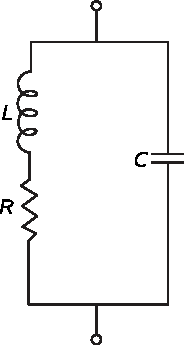
\includegraphics[width=0.3\linewidth]{fyz_fig0583.pdf}
      \caption{
               (\cite[s.~707]{Feynman02})}
      \label{fyz:fig0583}
    \end{figure}

    \begin{figure}[ht!]
      \centering
      \subcaptionbox{\label{fyz:fig0584a}}{\luafigure[0.3]{fyz_fig0584a.pdf}}
      \subcaptionbox{\label{fyz:fig0584b}}{\luafigure[0.3]{fyz_fig0584b.pdf}}
      \caption{
               (\cite[s.~748]{Feynman02})}
      \label{fyz:fig0584}
    \end{figure}

    pokus \ref{fyz:fig0584} nebo \ref{fyz:fig0584b}
    
    \begin{figure}[ht!]
      \centering
      \subcaptionbox{\label{fyz:fig0585a}}{\luafigure[0.3]{fyz_fig0585a.pdf}}
      \subcaptionbox{\label{fyz:fig0585b}}{\luafigure[0.3]{fyz_fig0585b.pdf}}
      \subcaptionbox{\label{fyz:fig0585c}}{\luafigure[0.3]{fyz_fig0585c.pdf}}
      \label{fyz:fig0585}
      \caption{
               (\cite[s.~748]{Feynman02})}
    \end{figure}

    \begin{figure}[ht!] %\ref{fyz:fig0586}
      \centering
      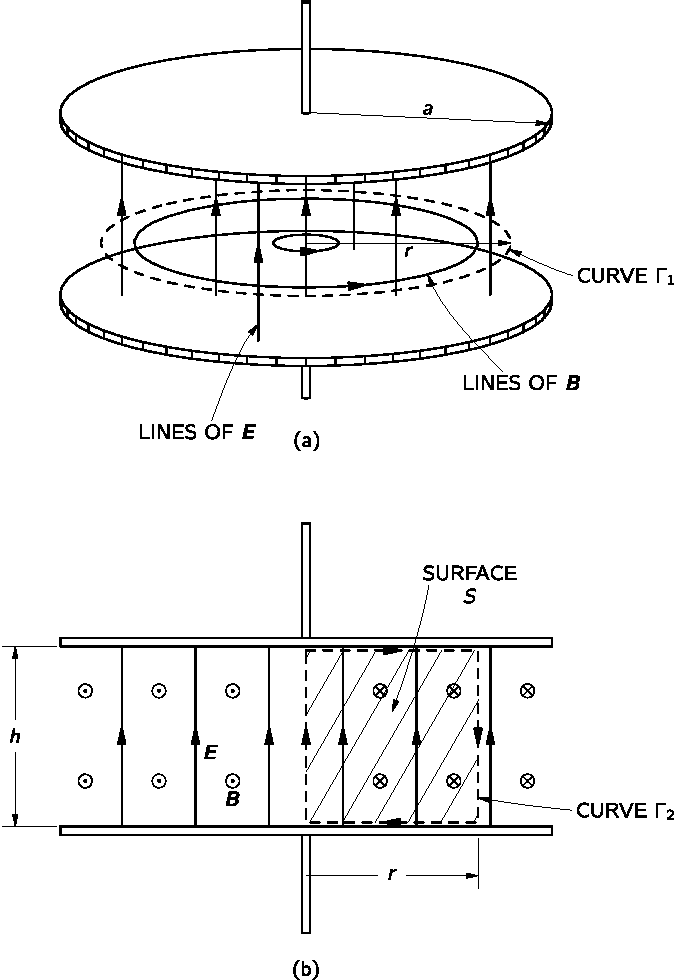
\includegraphics[width=0.7\linewidth]{fyz_fig0586.pdf}
      \caption{
               (\cite[s.~707]{Feynman02})}
      \label{fyz:fig0586}
    \end{figure}
    
    \begin{figure}[ht!] %\ref{fyz:fig0587}
      \centering
      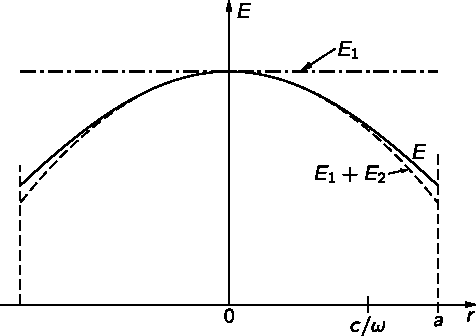
\includegraphics[width=0.7\linewidth]{fyz_fig0587.pdf}
      \caption{
               (\cite[s.~707]{Feynman02})}
      \label{fyz:fig0587}
    \end{figure}

    \begin{figure}[ht!] %\ref{fyz:fig0588}
      \centering
      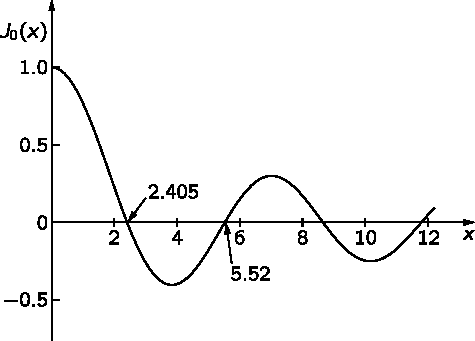
\includegraphics[width=0.7\linewidth]{fyz_fig0588.pdf}
      \caption{
               (\cite[s.~707]{Feynman02})}
      \label{fyz:fig0588}
    \end{figure}

    \begin{figure}[ht!]
      \centering
      \subcaptionbox{\label{fyz:fig0589a}}{\luafigure[0.7]{fyz_fig0589a.pdf}}               \\
      \subcaptionbox{\label{fyz:fig0589b}}{\luafigure[0.7]{fyz_fig0589b.pdf}}              
      \caption{Pohyb tekutiny v proudové trubici
               (\cite[s.~748]{Feynman02})}
    \end{figure}

    \begin{figure}[ht!] %\ref{fyz:fig0590}
      \centering
      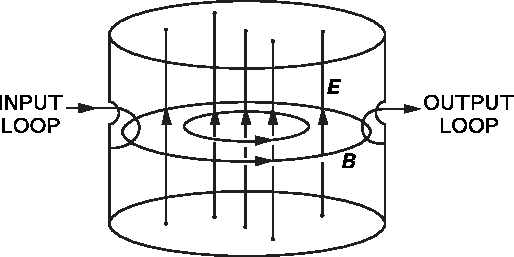
\includegraphics[width=0.7\linewidth]{fyz_fig0590.pdf}
      \caption{
               (\cite[s.~707]{Feynman02})}
      \label{fyz:fig0590}
    \end{figure}
    
    \begin{figure}[ht!] %\ref{fyz:fig0591}
      \centering
      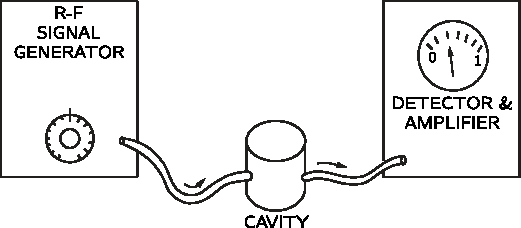
\includegraphics[width=0.7\linewidth]{fyz_fig0591.pdf}
      \caption{
               (\cite[s.~707]{Feynman02})}
      \label{fyz:fig0591}
    \end{figure}

    \begin{figure}[ht!] %\ref{fyz:fig0592}
      \centering
      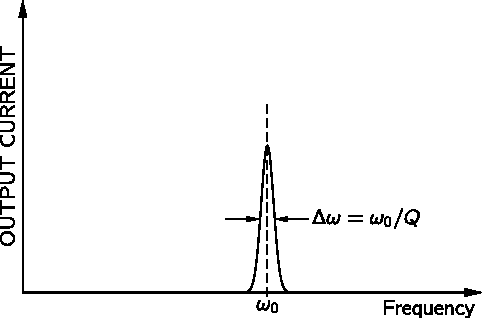
\includegraphics[width=0.7\linewidth]{fyz_fig0592.pdf}
      \caption{
               (\cite[s.~707]{Feynman02})}
      \label{fyz:fig0592}
    \end{figure}

    \begin{figure}[ht!] %\ref{fyz:fig0593}
      \centering
      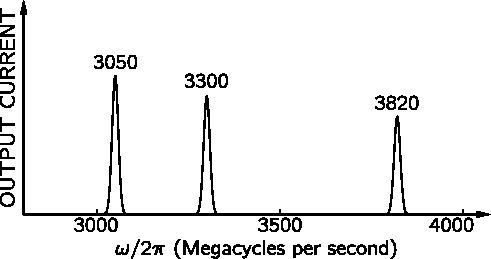
\includegraphics[width=0.7\linewidth]{fyz_fig0593.pdf}
      \caption{
               (\cite[s.~707]{Feynman02})}
      \label{fyz:fig0593}
    \end{figure}

    \begin{figure}[ht!]
      \centering
      \subcaptionbox{\label{fyz:fig0594a}}{\luafigure[0.5]{fyz_fig0594a.pdf}}               \\
      \subcaptionbox{\label{fyz:fig0594b}}{\luafigure[0.5]{fyz_fig0594b.pdf}}              
      \caption{
               (\cite[s.~748]{Feynman02})}
    \end{figure}

    \begin{figure}[ht!] %\ref{fyz:fig0595}
      \centering
      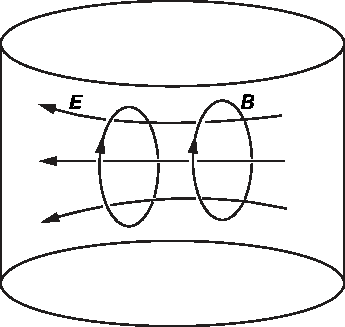
\includegraphics[width=0.5\linewidth]{fyz_fig0595.pdf}
      \caption{
               (\cite[s.~707]{Feynman02})}
      \label{fyz:fig0595}
    \end{figure}

    \begin{figure}[ht!] %\ref{fyz:fig0596}
      \centering
      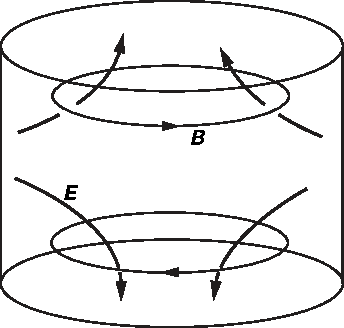
\includegraphics[width=0.5\linewidth]{fyz_fig0596.pdf}
      \caption{
               (\cite[s.~707]{Feynman02})}
      \label{fyz:fig0596}
    \end{figure}

    \begin{figure}[ht!]
      \centering
      \subcaptionbox{\label{fyz:fig0597a}}{\luafigure[0.45]{fyz_fig0597a.pdf}}
      \subcaptionbox{\label{fyz:fig0597b}}{\luafigure[0.45]{fyz_fig0597b.pdf}}               \\
      \subcaptionbox{\label{fyz:fig0597c}}{\luafigure[0.45]{fyz_fig0597c.pdf}}
      \caption{
               (\cite[s.~748]{Feynman02})}
      \label{fyz:fig0597}
    \end{figure}

    \begin{figure}[ht!]
      \centering
      \subcaptionbox{\label{fyz:fig0598a}}{\luafigure[0.6]{fyz_fig0598a.pdf}}               \\
      \subcaptionbox{\label{fyz:fig0598b}}{\luafigure[0.6]{fyz_fig0598b.pdf}}               \\
      \subcaptionbox{\label{fyz:fig0598c}}{\luafigure[0.7]{fyz_fig0598c.pdf}}
      \caption{
               (\cite[s.~748]{Feynman02})}
      \label{fyz:fig0598}
    \end{figure}

    \begin{figure}[ht!] %\ref{fyz:fig0599}
      \centering
      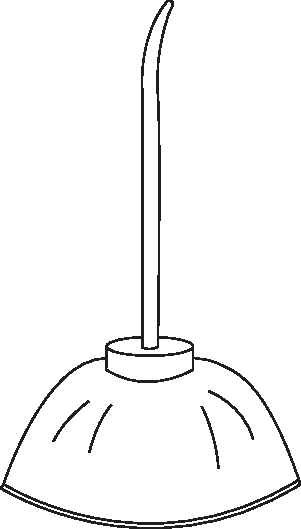
\includegraphics[width=0.3\linewidth]{fyz_fig0599.pdf}
      \caption{
               (\cite[s.~707]{Feynman02})}
      \label{fyz:fig0599}
    \end{figure}

    \todo[inline]{Kapitola fey2ch23 je nedodělaná, obsahuje pouze obrázky}
%} %tikzset
%~~~~~~~~~~~~~~~~~~~~~~~~~~~~~~~~~~~~~~~~~~~~~~~~~~~~~~~~~~~~~~~~~~~~~~~~~~~~~~~~~~~~~~~~~~~~~~~~~~
